
\section{Experiments}
\label{sec:experiments}
We evaluate \ours on three real-world contact-rich manipulation tasks. 
Our experiments are designed to answer three questions: whether multimodal visuo-tactile steering improves policy over unimodal guidance (Sec.~\ref{sec:exp_multimodal_guidance}); whether a learned latent world model and semantically aligned verifier provides reliable rewards for predicted outcomes (Sec.~\ref{sec:experiment_verifier}); and whether the proposed bi-level optimization balances performance and efficiency compared to naive visual-tactile fusion (Sec.~\ref{sec:experiment_bilevel}).


\textbf{Robot Setup, Tasks, and Data Collection.}
We use a Franka Emika robot with RGB and tactile sensors to evaluate \ours on three real-world contact-rich manipulation tasks, including \textit{wiping}, \textit{insertion}, and \textit{pipette transfer}. These tasks require both global visual reasoning, such as selecting the correct mark, hole, or target cup, and local tactile feedback for maintaining contact, resolving alignment, or stabilizing grasp and dispensing behavior. 
 For each task, we collect $50$ expert demonstrations to train the base diffusion policy $\policy$ with additional $250$ policy rollouts from intermediate policy checkpoints to train the visuo-tactile world model.  Details are in App~\ref{app:real_world_setup}.



\textbf{Base Policy.}
We train a diffusion policy that predicts a 16-step action chunk and executes the first $h=8$ actions at each step. For long-horizon lookahead $H=16$, we recursively roll out the visuo-tactile world model and condition the policy on predicted future observations. Our main experiments use a vision-conditioned policy $\pi_\theta(\action \mid \obsv_t)$; App~\ref{app:visuo_tactile_policy} evaluates a visuo-tactile policy $\pi_\theta(\action \mid \obsv_t,\obst_t)$.




\textbf{World Model and Verifiers.}
We train separate visual and tactile decoders, and a transformer-based latent dynamics model for visuo-tactile prediction. For steering, we modify ROBOMETER~\cite{liang2026robometer} with KV caching for online visual reward estimation, and compute tactile rewards by comparing pretrained tactile embeddings~\cite{fenganytouch2} with CLIP text embeddings~\cite{radford2021learning}. Details are in App~\ref{app:implement_visuo_tactile_world_model} -~\ref{app:implement_tactile_steering}.



\begin{figure}[!ht]
\vspace{-0.4cm}
    \centering
    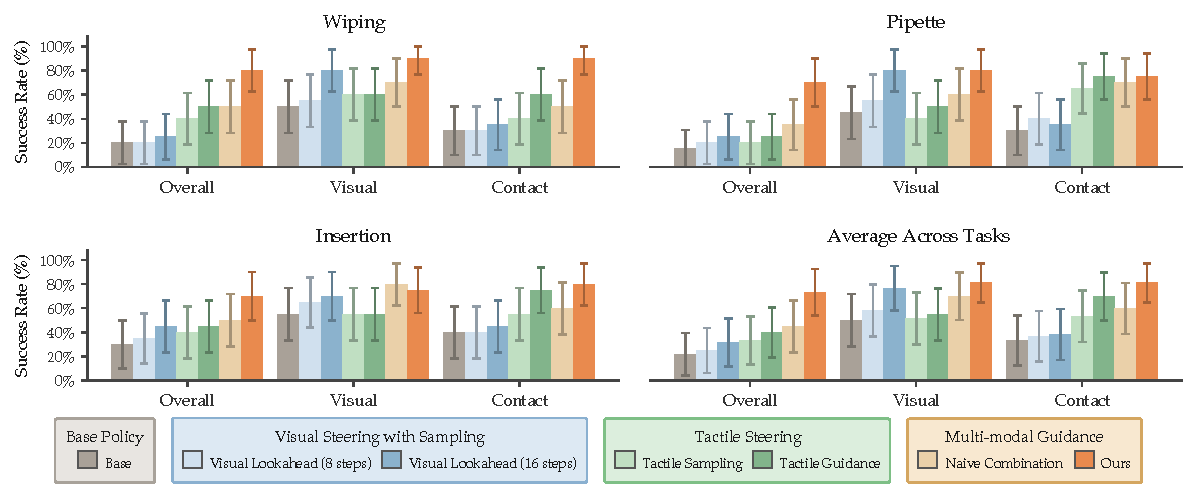
\includegraphics[width=\linewidth]{figures/policy_performance_2x2_v5.pdf}
   \caption{\textbf{Policy Steering Performance}. \ours outperforms vision-only, tactile-only, and naive multimodal baselines across three tasks. Error bars show binomial standard errors over $20$ trials.}
    \vspace{-0.2cm}
    \label{fig:policy_success_rate}
\end{figure}

\subsection{Multi-Modal Visuo-Tactile Steering Outperforms Single-Modality Steering}
\label{sec:exp_multimodal_guidance}
We compare our multi-modal guidance \ours against five methods in Fig.~\ref{fig:policy_success_rate}: 1) 
\textbf{Base Policy}; 2) visual steering, including
\textbf{Visual Lookahead (8 steps) vs (16 steps)}, which selects the best of $N=10$ with visual verifier over different prediction horizons; 3) tactile steering, including
\textbf{Tactile Sampling}, which selects the best of $N=10$ samples with tactile verifier; 
\textbf{Tactile Guidance}, classifier-based tactile guidance;  
We omit classifier-based visual guidance due to the reasons discussed in Sec.~\ref{subsec:method_bilevel_execution}.
We report \textbf{Overall}, \textbf{Visual}, and \textbf{Contact} success, measuring full task completion, correct visual goal following, and appropriate local physical interaction, respectively.





\paras{Results}
In Fig.~\ref{fig:policy_success_rate}, visual-only steering improves visual success but provides limited gains in overall task completion, while tactile-only steering improves contact behavior without reliably satisfying the task goal. In contrast, \ours jointly improves visual and contact success, leading to a $51\%$ increase in overall task success over base policy and at least 33\% gain over unimodal baselines.

Fig.~\ref{fig:multimodal_failure_modes} illustrates why multimodal steering is particularly helpful in the pipette task: vision-only steering can choose globally plausible but imprecise actions (e.g., spilling), while tactile-only steering can improve local contact with adequate grasp force but it misses the intended visual goal. 
Our multimodal method succeeds by satisfying both local and global performance requirements. More qualitative results for other tasks are provided in App~\ref{app:results_multi_modal}.





















\begin{figure}[t]
    \centering
    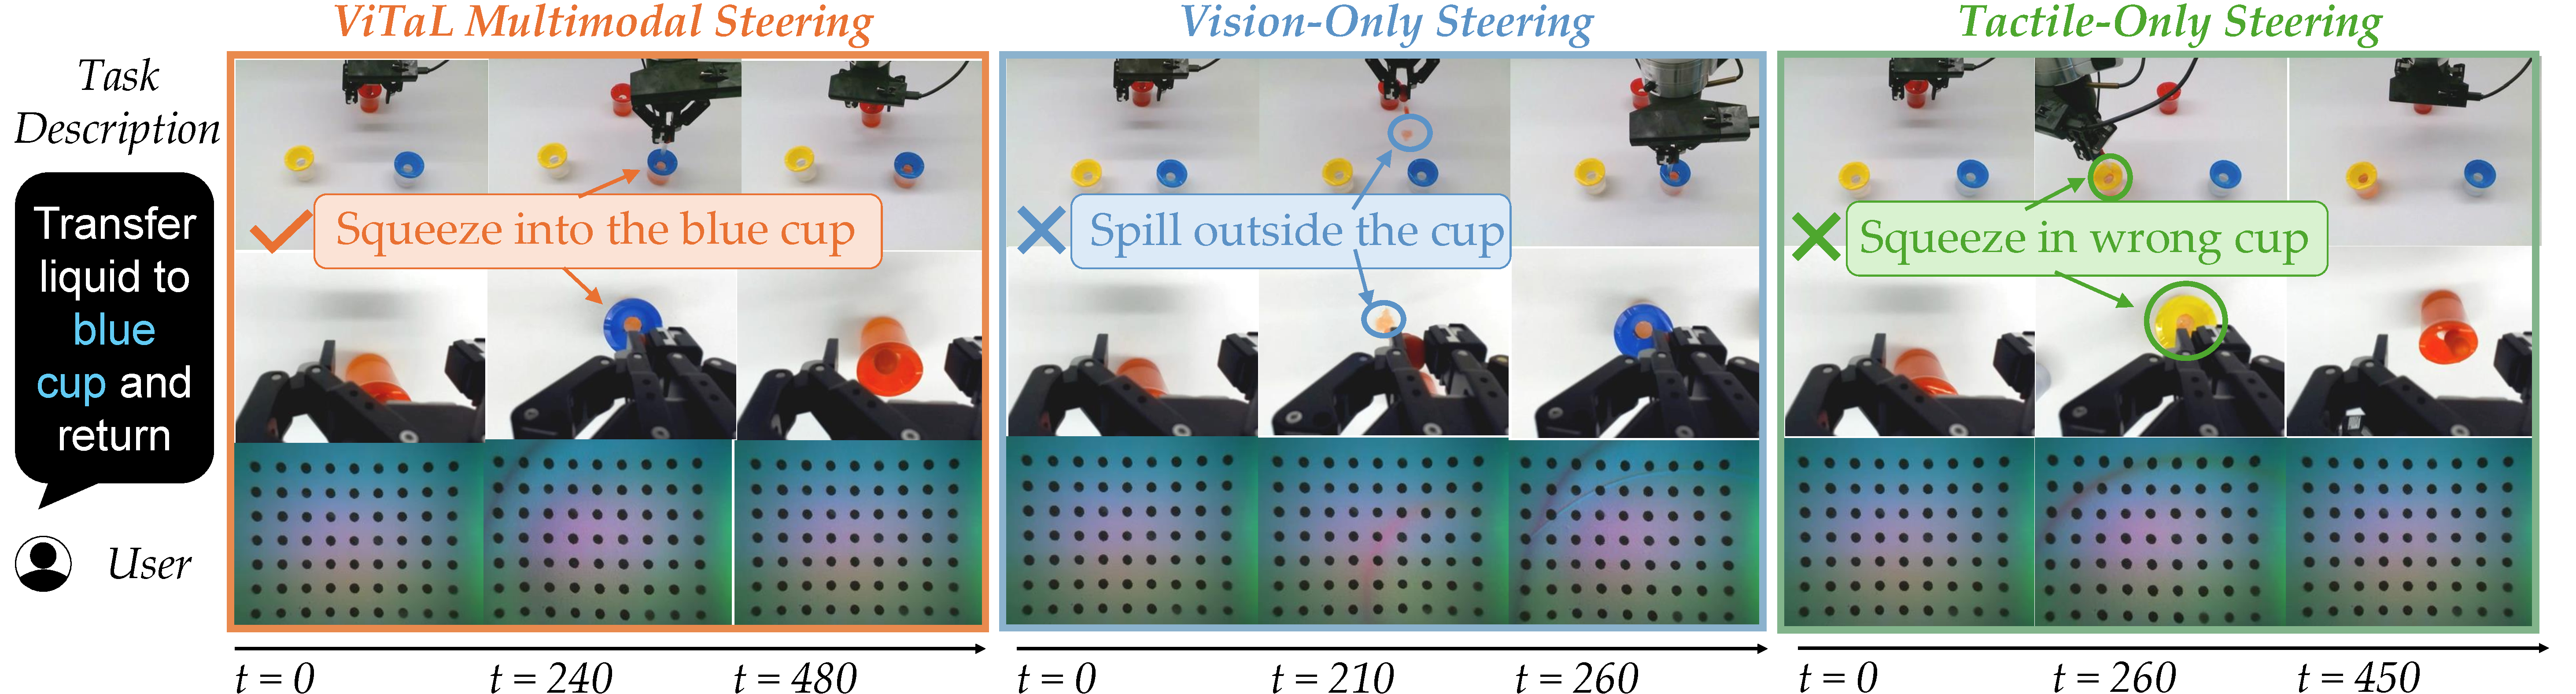
\includegraphics[width=0.95\linewidth]{figures/corl_qualitative_multi_modal_corl_v7.pdf}
    \caption{
    \textbf{Policy Steering with Different Guidance Modalities}. Vision-only Steering (middle) fails due to local contact errors, while tactile-only steering (right) can fail due to global task misalignment. \ours (left) with multimodal steering addresses both failure modes.
    }
    \vspace{-0.4cm}\label{fig:multimodal_failure_modes}
\end{figure}

\begin{table}[t]
\centering
\tiny
\caption{
\textbf{Reward Accuracy}. We evaluate reward with preference-order accuracy. GT versus Pred uses ground-truth versus predicted futures. Error bars show binomial standard errors over $40$ trials.
}
\label{tab:reward_eval}
\resizebox{0.95\linewidth}{!}{
\begin{tabular}{lcccccccc}
\toprule
\multirow{2}{*}{\textbf{Src.}}
& \multicolumn{4}{c}{\textbf{Visual Reward (\%)}} 
& \multicolumn{4}{c}{\textbf{Tactile Reward (\%)}} \\
\cmidrule(lr){2-5}
\cmidrule(lr){6-9}
& \textbf{Wiping} & \textbf{Insertion} & \textbf{Pipette} & \textbf{Avg.}
& \textbf{Wiping} & \textbf{Insertion} & \textbf{Pipette} & \textbf{Avg.} \\
\midrule
GT
& $80.0{\pm}6.3$ & $70.0{\pm}7.2$ & $\mathbf{100.0{\pm}0.0}$ & $83.3{\pm}5.9$
& $85.0{\pm}5.6$ & $70.0{\pm}7.2$ & $\mathbf{80.0{\pm}6.3}$ & $78.3{\pm}6.5$ \\
Pred
& $\mathbf{82.5{\pm}6.0}$ & $\mathbf{72.5{\pm}7.1}$ & $\mathbf{100.0{\pm}0.0}$ & $\mathbf{85.0{\pm}5.6}$
& $\mathbf{90.0{\pm}4.7}$ & $\mathbf{77.5{\pm}6.6}$ & $77.5{\pm}6.6$ & $\mathbf{81.7{\pm}6.1}$ \\
\bottomrule
\end{tabular}
}
\vspace{-0.4cm}
\end{table}
\subsection{Semantically-Aligned Visual and Tactile Verifiers Enable Global and Local Adaptation}
\label{sec:experiment_verifier}

Effective steering requires accurately predicting \textit{both} visuo-tactile outcomes and their respective rewards. Thus, we evaluate whether our visual and tactile verifiers provide reliable semantic rewards for steering predicted futures. 
We first compare our joint visuo-tactile world model against separately trained unimodal ones with standard visual metrics and tactile-related metrics. For brevity, these world models results are in App~\ref{app:world_model_ablation} and we focus on the reward model results in this section. However, Fig.~\ref{fig:reward_qualitative} visualizes the decoded visual and tactile world model predictions in the pipette task.

\para{Metrics} We focus on evaluating reward quality of both ground-truth observations (\textbf{GT}) and world-model predictions (\textbf{Pred}) with preference-order accuracy~\cite{tian2026position} shown in App.~\ref{app:results_reward_world_model}. For each task, we select rollout pairs with different human preferences, rank each pair by the sum of predicted reward divided by rollout length, and measure how often the predicted order matches the human order.


\para{Results}
Table~\ref{tab:reward_eval} shows that both the ROBOMETER visual reward and our tactile reward achieve at least $70\%$ preference-order accuracy across tasks on both \textbf{GT} and \textbf{Pred} observations. In some cases, \textbf{Pred} rewards are slightly more accurate, likely because predicted latents smooth observation noise (Fig.~\ref{fig:reward_qualitative} right) and are easier to rank due to lower visual/tactile variations than real rollouts.

Fig.~\ref{fig:reward_qualitative} further illustrates the semantic alignment of both verifiers on the pipette task. The visual verifier assigns higher reward when the robot dispenses into the cup that matches the target cup specified in textual description (e.g, the yellow cup), and phase-level textual objectives focus on the alignment to the relevant subgoal (e.g. transfer to the target cup or move back to the red cup). The tactile verifier captures the transition from gentle to firm grasp, consistent with marker-tracking force estimates. Together, these results show that our visual rewards can identify global goal satisfaction, while our proposed tactile rewards provide meaningful local contact signals.










\begin{figure}
    \centering
    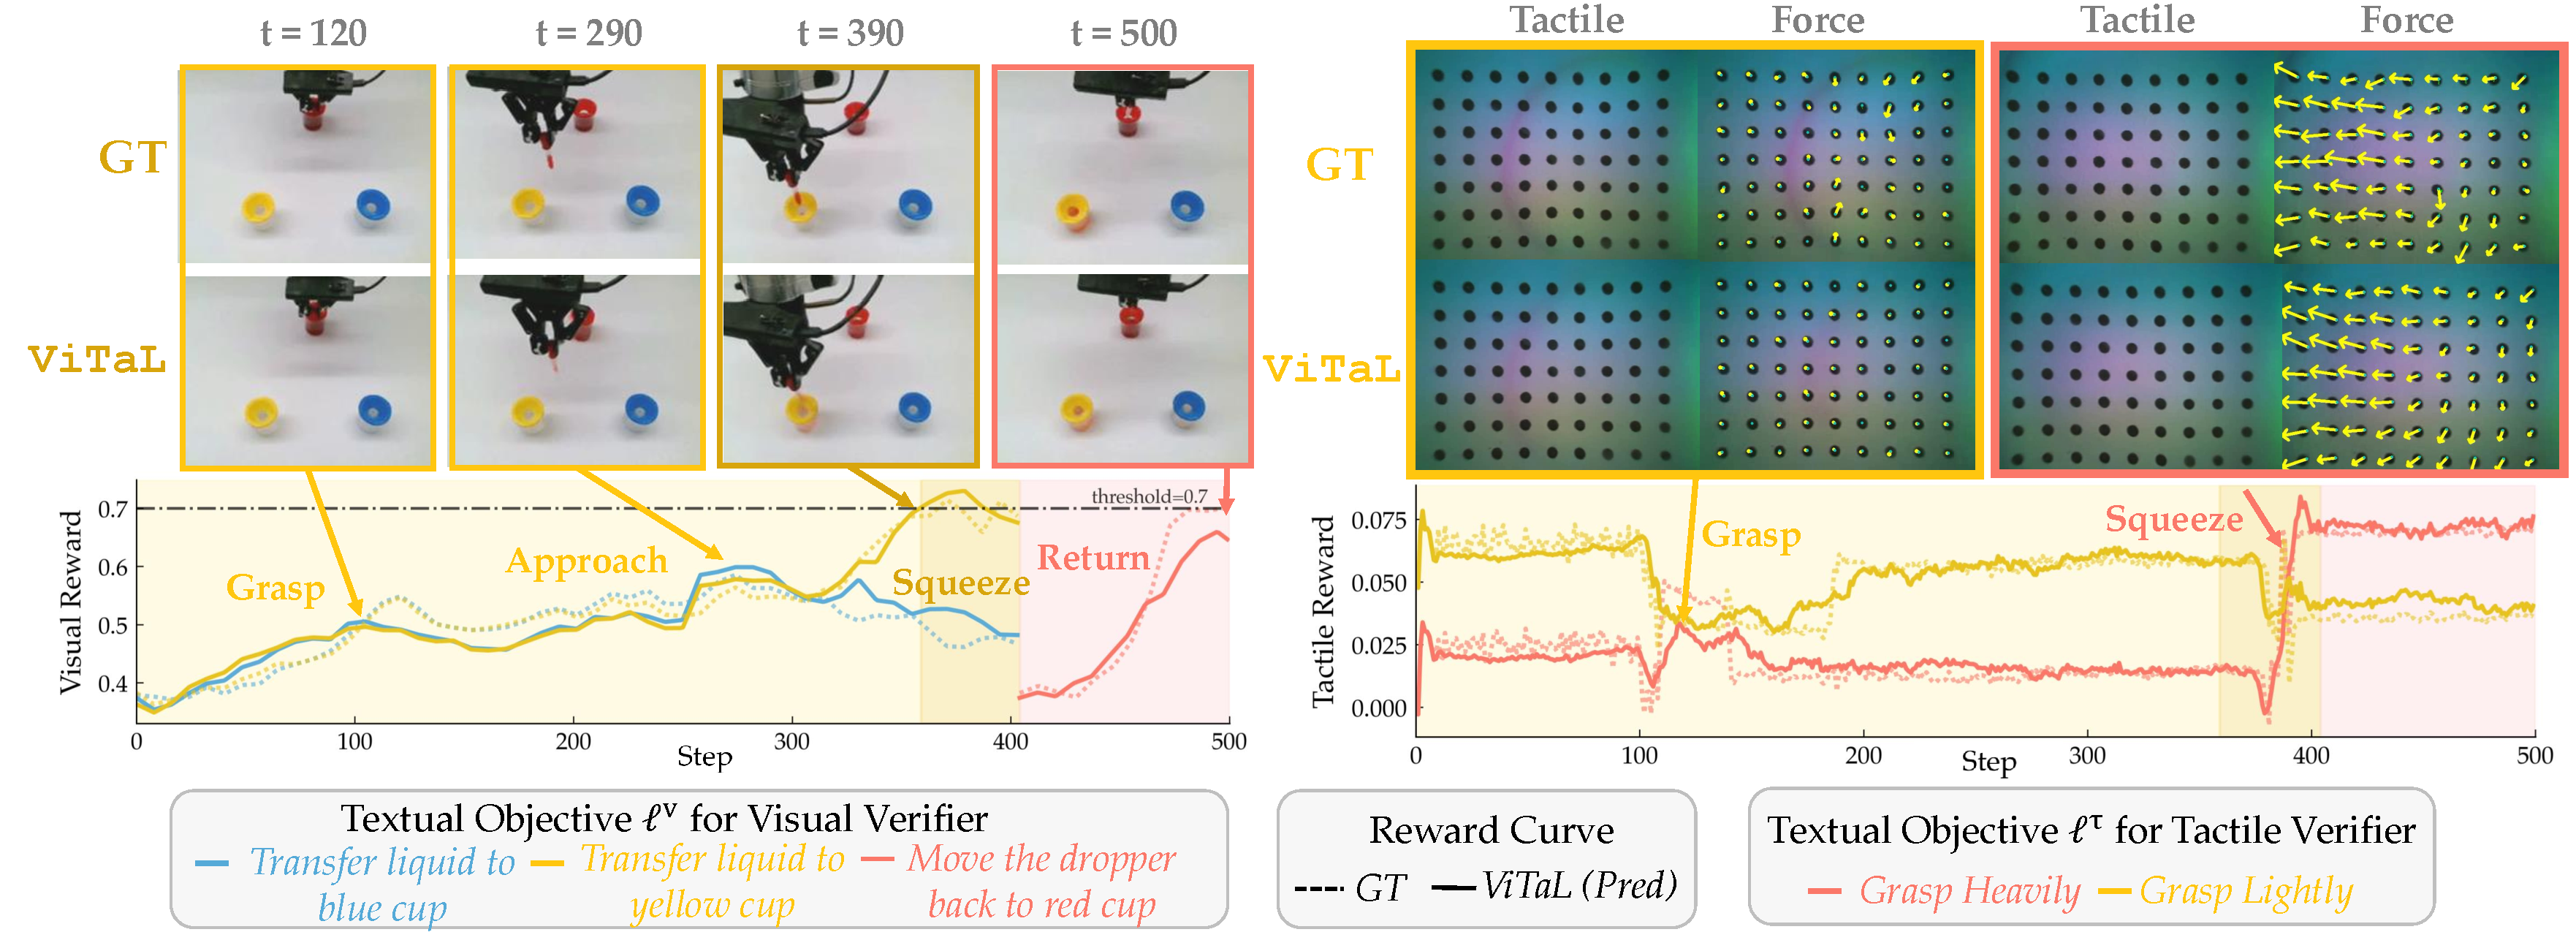
\includegraphics[width=0.9\linewidth]{figures/reward_plot_corl_v4.pdf}
    \caption{
\textbf{Visual and Tactile Verification.}
Our visual verifier (left) identifies whether the target cup is selected and the phase transition, while the tactile verifier (right) captures changes in grasp force.
}
  \vspace{-0.3cm}\label{fig:reward_qualitative}
\end{figure}
\begin{figure}
    \centering
    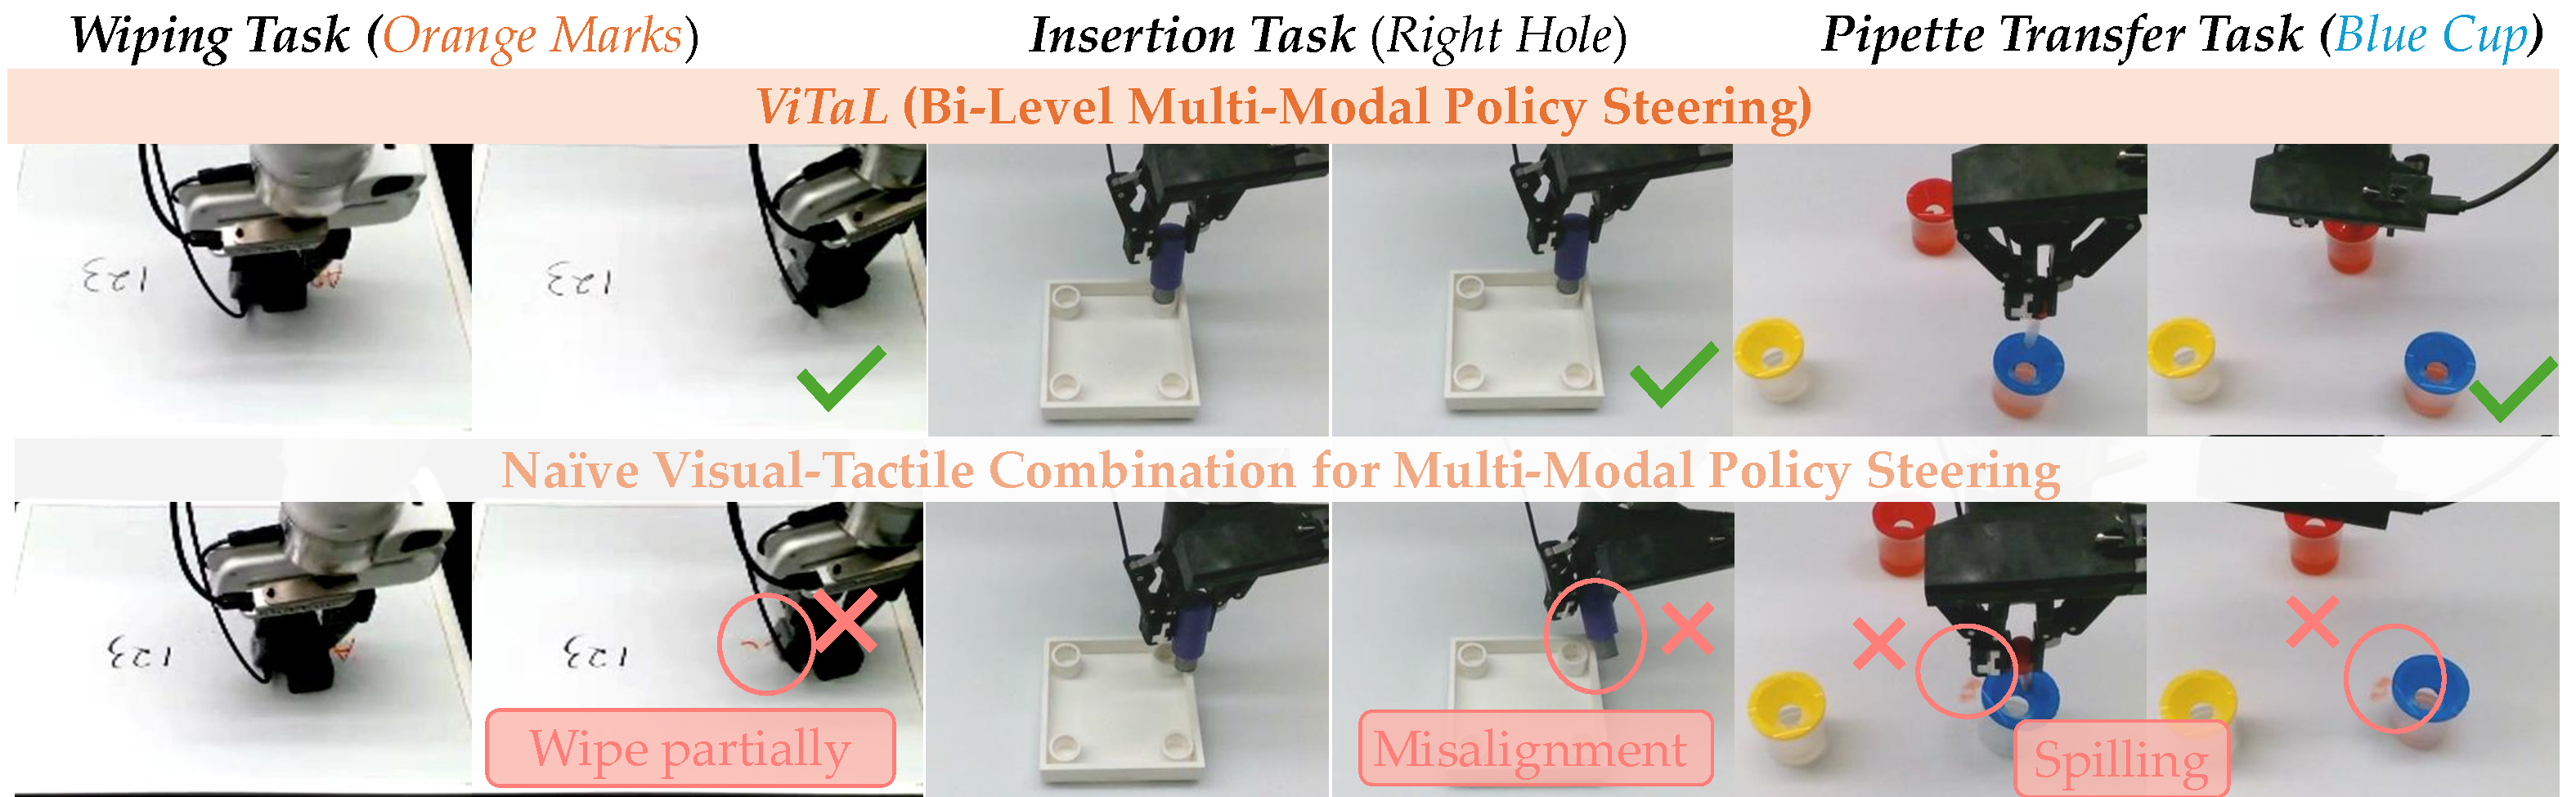
\includegraphics[width=0.9\linewidth]{figures/bilevel_policy_performance_corl_v4.pdf}
    \caption{\textbf{Multi-Modal Policy Steering}. \ours (top) successfully completes three contact-rich tasks while naive combination (bottom) of both modalities during steering always fails.}
    \vspace{-0.cm}\label{fig:bilevel_qualitative}
\end{figure}

\subsection{Bi-Level Steering Achieves Balance Between Performance and Inference Speed}
\label{sec:experiment_bilevel}

We evaluate whether \ours achieves a better trade-off between task success and inference speed than naive multimodal fusion. We compare \textbf{Base Policy}; \textbf{Naive Combination}, which normalizes visual and tactile rewards separately across $N=10$ samples and sums them for action selection; and \ours, which first selects actions using long-horizon visual lookahead and then refines it with local tactile guidance. We report \textbf{Overall}, \textbf{Visual}, and \textbf{Contact} success as in Sec.~\ref{sec:exp_multimodal_guidance}, together with inference-time overhead, to assess whether \ours improves steering without sacrificing efficiency.

\para{Results}
As shown in Fig.~\ref{fig:policy_success_rate}, \ours outperforms \textbf{Naive Combination} by at least $20\%$ across all three tasks. Naive reward fusion often suffers from reward imbalance: the visual objective can dominate selection, leading to actions that appear globally plausible but fail to establish proper contact. Fig.~\ref{fig:bilevel_qualitative} illustrates these failures, where naive fusion can leave orange marks partially wiped, misalign the peg with the hole, or spill liquid. In contrast, \ours uses vision to efficiently select globally appropriate behaviors and touch to make targeted local corrections. As detailed in App.~\ref{app:results_bi_level}, \ours adds $0.05$ second per policy inference step (8 actions) over naive fusion while yielding substantially higher success. These results show that bi-level steering provides a stronger success--speed trade-off.









































